\documentclass[11pt]{article}

\input{../shared/preamble.tex}

\usepackage{amsmath}
\usepackage{graphicx}
\usepackage{cleveref}

\title{Winning Probabilities as Credit:\\
       Fast, Redundancy-Aware Attribution}
\author{Peter Cotton}
\date{\today}

\newcommand{\E}{\mathbb{E}}
\newcommand{\Prob}{\mathbb{P}}
\newcommand{\R}{\mathbb{R}}
\DeclareMathOperator*{\argmaxop}{arg\,max}

\newtheorem{theorem}{Theorem}
\newtheorem{proposition}{Proposition}
\newtheorem{definition}{Definition}

\begin{document}
\maketitle

\begin{abstract}
The probability that a competitor wins a noisy race---the Thurstonian choice
probability, equivalently the gradient of an expected-maximum potential---is a
rule for attributing credit among correlated contributors. It is efficient and
symmetric (two of the Shapley axioms), it is \emph{redundancy-aware} (contributors
that move together share a single contributor's credit rather than double-counting),
it is differentiable in the contributors' abilities, it updates online, and it
costs $O(Mn)$ in a single Monte-Carlo pass with no coalition enumeration. We place
it next to the Shapley value: on the expected-maximum game its \emph{diagonal
integral} is an Aumann--Shapley value, but the winning probability itself is a
distinct, gradient-valued object, not the Shapley value of the membership game---a
cousin, not a drop-in. The practical separation is computational: redundancy-aware
credit in one linear pass where exact Shapley is $O(2^n)$ and sampled Shapley is
$O(RMn)$ with $1/\sqrt R$ error. We show that the headline redundancy property---an
even split of credit among near-duplicates---is a property of the \emph{calibrated}
equal-ability race rather than of raw scores, and we demonstrate the rule on
forecast combination and feature attribution. This develops the credit reading of
the construction in the companion paper on Thurstone portfolios.
\end{abstract}

\section{Introduction}
\label{sec:intro}

Attributing credit for a collective outcome among contributors that overlap is an
old problem with a canonical answer, the Shapley value \parencite{shapley1953}, and
a canonical difficulty, its cost: the exact value sums marginal contributions over
all $2^n$ coalitions, and the practical estimators sample permutations
\parencite{strumbelj2014} or, in machine learning, fit a local surrogate (SHAP,
\textcite{lundberg2017}). Correlated contributors compound the difficulty: a
contributor and a near-duplicate should \emph{share} credit, not each receive it in
full, and many cheap importance measures (marginal screening, regression
coefficients, permutation importance) either double-count the pair or split it
arbitrarily.

We study a different credit rule with a single, cheap evaluation. Give each
contributor $i$ a latent ability $\theta_i$ and a noisy performance
$X_i = \theta_i + \eta_i$ under a joint law $S$; the credit of $i$ is the
probability that it wins,
\begin{equation}
  w_i \;=\; \Prob\!\Big( X_i = \max_j X_j \Big).
  \label{eq:winprob}
\end{equation}
This is the Thurstonian choice probability, and the vector $w = W_S(\theta)$ is the
gradient of an expected-maximum potential (\Cref{sec:rule}). Read as credit it has
three things going for it at once. It is redundancy-aware by construction: two
contributors that move together compete with \emph{each other}, so a co-moving pair
collapses toward a single winner and shares one contributor's credit. It is
differentiable in $\theta$, so it composes with gradient-based learning. And it
costs one Monte-Carlo pass, $O(Mn)$, returning all $n$ shares at once with no
coalition enumeration.

Our contributions are (i) the precise relationship to the Shapley value: the
winning probability is the gradient of the same expected-maximum potential whose
\emph{diagonal integral} is an Aumann--Shapley value
\parencite{owen1972, aumannshapley1974}, but it is not itself the Shapley value of
the membership game (\Cref{sec:shapley}); (ii) the computational separation,
$O(Mn)$ versus $O(2^n)$, quantified (\Cref{sec:complexity}); and (iii) the
clarification that the headline redundancy property---an \emph{even} split among
near-duplicates---belongs to the \emph{calibrated} equal-ability race, not to raw
contribution scores (\Cref{sec:redundancy}). We close with two applications,
forecast combination and feature attribution (\Cref{sec:apps}).

\section{The credit rule}
\label{sec:rule}

Let $S$ be a centered joint law on $\R^n$ (the \emph{simulation}) and define the
expected-maximum potential and its gradient,
\begin{equation}
  G_S(\theta) \;=\; \E_{\eta\sim S}\Big[\max_i (\theta_i + \eta_i)\Big],
  \qquad
  W_S(\theta) \;=\; \nabla G_S(\theta) \in \Delta,
  \label{eq:potential}
\end{equation}
where $\Delta$ is the simplex. When $S$ has a density the maximizer is a.s.\ unique,
$G_S$ is smooth and convex, and $\nabla_i G_S(\theta) = \Prob(i = \argmaxop_j
X_j) = w_i$, recovering \eqref{eq:winprob}; this is the Williams--Daly--Zachary /
perturbed-maximum identity \parencite{williams1977, mcfadden1981, berthet2020}.
Because $G_S(\theta + c\mathbf 1) = G_S(\theta) + c$, gradients and Jacobians live
on the tangent space $T\Delta = \{v : \mathbf 1^\top v = 0\}$.

To use \eqref{eq:winprob} as an attribution we must fix the abilities. Given a
\emph{benchmark} $w^0 \in \operatorname{int}\Delta$ of marginal credits and a
reference law $S_0$, calibration inverts the gradient map,
\begin{equation}
  \theta^0 \;=\; W_{S_0}^{-1}(w^0) \quad (\text{mod } \mathbf 1),
  \label{eq:calib}
\end{equation}
which is well posed: for Gaussian $S_0 = \mathcal N(0, C_0)$ with $C_0 \succ 0$ the
map $W_{C_0} : \R^n/\!\operatorname{span}\{\mathbf 1\} \to \operatorname{int}\Delta$
is a smooth bijection, and the diagonal case admits a linear-time, Monte-Carlo-free
inverse (the Fast Ability Transform, \textcite{cotton2021}). The credit rule is then
\begin{equation}
  T_{S_0\to S_1}(w^0) \;=\; W_{S_1}\!\big(W_{S_0}^{-1}(w^0)\big),
  \label{eq:tilt}
\end{equation}
the winning probabilities of the same abilities re-evaluated under a
dependence-rich law $S_1$. With $S_1 = S_0$ the benchmark is reproduced; with $S_1$
carrying the contributors' empirical dependence, \eqref{eq:tilt} re-weights the
benchmark for redundancy.

\section{Relationship to the Shapley value}
\label{sec:shapley}

Both the winning probability and the Shapley value can distribute the same
quantity. Take the cooperative game
\begin{equation}
  v(\mathcal S) \;=\; \E\Big[\max_{i\in\mathcal S} X_i\Big],
  \qquad v(\varnothing) = 0,
  \label{eq:game}
\end{equation}
whose grand value $v(N) = \E[\max_i X_i] = G_S(\theta)$. The winning-probability
vector and the Shapley value of \eqref{eq:game} both lie on the simplex (after
normalization) and both satisfy two Shapley axioms: \emph{efficiency} (the shares
sum to the total) and \emph{symmetry} (interchangeable contributors receive equal
credit). They differ on the third.

\begin{proposition}[Gradient versus coalitional value]
\label{prop:bridge}
Let $G_S$ be differentiable. Then $w = \nabla G_S(\theta)$ is the marginal of the
grand coalition, while the Shapley value of \eqref{eq:game} is the average marginal
over all sub-coalitions; equivalently (Owen's multilinear extension
\parencite{owen1972}) it is the diagonal integral $\phi_i = \int_0^1 \partial_i
F(t\mathbf 1)\,dt$ of the extension $F$. Consequently the winning probability is the
diagonal-path \emph{integrand}, and its own diagonal integral
$\mathrm{AS}_i = \theta_i\!\int_0^1 W_S(t\theta)_i\,dt$ is the Aumann--Shapley value
\parencite{aumannshapley1974} of the ability-scaling game $f(t) = G_S(t\!\cdot\!
\theta)$, which is efficient and symmetric.
\end{proposition}

Numerically (\Cref{tab:shapley}): on a small game the identity $w = \nabla G_S$
holds to Monte-Carlo error; the diagonal integral is efficient and symmetric to the
same; and the winning probability differs from the membership-game Shapley value,
in a direction that depends on the field. So the winning probability is a
\emph{cousin} of the Shapley value---an exact Aumann--Shapley value of the ability
game, sharing efficiency and symmetry---but not a drop-in for the membership-game
value. % TODO: state the AS identity as a proper theorem with proof.

\begin{table}[h]
  \centering
  \caption{Five-contributor game (contributors $3,4$ an exchangeable near-duplicate
  pair). The gradient identity holds; the diagonal integral is an efficient,
  symmetric Aumann--Shapley value; the winning probability is not the
  membership-game Shapley value. From \texttt{experiments/shapley\_bridge.py}.}
  \label{tab:shapley}
  \begin{tabular}{lc}
    \toprule
    Check & Result \\
    \midrule
    $\max_i |w_i - \partial_i G_S|$ (gradient identity)      & $7\times10^{-5}$ \\
    $|\sum_i \mathrm{AS}_i - (G_S(\theta)-G_S(0))|$ (efficiency) & $2\times10^{-6}$ \\
    $|\mathrm{AS}_3 - \mathrm{AS}_4|$ (symmetry)             & $3\times10^{-4}$ \\
    $\max_i |\,\text{Shapley}_i - w_i|$ (cousin, not equal)  & $1.5\times10^{-2}$ \\
    \bottomrule
  \end{tabular}
\end{table}

\section{Computational complexity}
\label{sec:complexity}

The practical case for the winning probability as credit is its cost. All three
schemes target a redundancy-aware split over $n$ contributors of the game
\eqref{eq:game}:
\begin{itemize}
  \item exact Shapley enumerates $2^n$ coalitions;
  \item sampled Shapley averages $R$ random permutations of running-maximum
        marginals, $O(RMn)$, with error $O(1/\sqrt R)$;
  \item the race takes one $\argmaxop$ sweep of $M$ draws, $O(Mn)$, returning all
        $n$ shares at once and exact in $M$.
\end{itemize}

\begin{figure}[h]
  \centering
  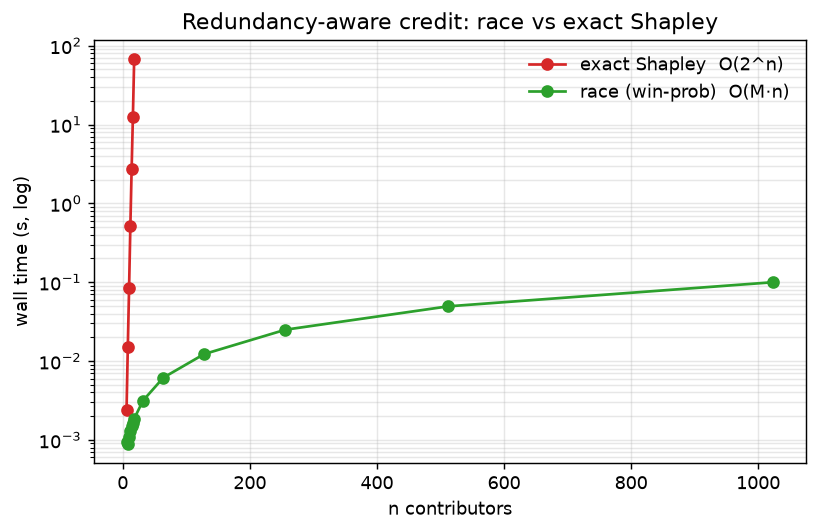
\includegraphics[width=0.66\textwidth]{figures/shapley_complexity.png}
  \caption{Wall time for redundancy-aware credit on $n$ contributors. Exact Shapley
  doubles per contributor (red); the race is flat in $n$ at the same resolution
  (green) and returns all shares in one pass. From
  \texttt{experiments/shapley\_complexity.py}.}
  \label{fig:complexity}
\end{figure}

At $n=12$ exact Shapley takes $4.8$\,s, sampled Shapley ($R{=}200$) $100$\,ms at
$\pm0.03$ accuracy, and the race $0.2$\,ms---four to five orders of magnitude
(\Cref{fig:complexity}). Exact Shapley doubles per added contributor ($67$\,s at
$n=18$; extrapolating, $\sim\!9$ years at $n=40$); the race is flat at $\sim0.2$\,ms
and handles $n=5000$ in $57$\,ms, where $2^{5000}$ coalitions is not a number one
writes down. The race is the gradient of the same potential delivered in a single
linear pass, and it is differentiable and online; none of these hold for the
combinatorial value.

\section{Redundancy, and the calibration condition}
\label{sec:redundancy}

The reason to prefer this credit rule over a correlation-blind one is redundancy.

\begin{proposition}[Redundancy consistency at fixed abilities]
\label{prop:redundancy}
If contributors $i,j$ have equal ability and comonotone performances, then either
wins exactly when the other does; with symmetric tie-splitting each receives half
of the single-contributor winning probability, and the pair's combined credit
equals that of one contributor.
\end{proposition}

This is a property of the race \emph{at fixed, equal abilities}. It does not follow
for an arbitrary vector of scores fed through $\argmaxop$: if near-duplicates carry
slightly unequal scores, the largest wins almost every draw and the split is
winner-take-all. The fix is calibration \eqref{eq:calib}: set the benchmark $w^0$ to
the contributors' \emph{marginal} credit---equal across genuine duplicates---then
tilt under their empirical dependence, so the pair is de-duplicated and split
evenly. \Cref{tab:redundancy} shows both regimes on a feature-attribution task: a
signal direction present as six near-duplicate columns plus twenty noise features.
Raw $\argmaxop$ is winner-take-all (copy spread $26\times$); the calibrated race
splits the copies evenly (spread $1.1$), at a cost that is still far below
model-agnostic SHAP.

\begin{table}[h]
  \centering
  \caption{Feature attribution: one signal direction as six near-duplicate columns
  $+$ twenty noise features. ``Copy spread'' is the max/min credit across the six
  copies ($1$ is an even split). From \texttt{experiments/feature\_attribution.py}.}
  \label{tab:redundancy}
  \begin{tabular}{lcccc}
    \toprule
    Method & Signal cluster & Noise total & Copy spread & Time \\
    \midrule
    permutation importance       & $0.998$ & $0.002$ & $2.3$  & $41$\,ms \\
    mean $|\text{SHAP}|$          & $0.937$ & $0.063$ & $1.5$  & $0.3$\,ms \\
    race (raw $\argmaxop$)        & $0.998$ & $0.002$ & $26.5$ & $0.1$\,ms \\
    race (calibrated)             & $0.909$ & $0.091$ & $1.1$  & $0.3$\,s \\
    \bottomrule
  \end{tabular}
\end{table}

\section{Applications}
\label{sec:apps}

\paragraph{Forecast combination.}
Supplying the race with the base forecasters' per-period \emph{losses}
$L_{k,t}$ (so the lowest-loss forecaster wins) yields combination weights that are a
redundancy-aware credit split over models. On the M4 competition this is the
stable, small-sample member of the combination family; the companion paper reports
that study. The performance variable must be a loss, not a signed error, or the
``winner'' is merely the most negatively biased forecaster.

\paragraph{Feature attribution.}
\Cref{tab:redundancy} is the attribution use-case: a fast, redundancy-aware
importance. Raw scores give a quick screen but are winner-take-all among
correlates; the calibrated race delivers the even split that correlated-feature
attribution wants, at a fraction of SHAP's cost. The honest caveats are that
de-duplicated weight partly redistributes to weak contributors, and that the credit
is a share of wins, not an additive decomposition of a single prediction.

\section{Discussion}
\label{sec:discussion}

The winning probability is a fast, differentiable, online, redundancy-aware credit
rule---a cousin of the Shapley value with an exact Aumann--Shapley reading on the
ability game, and a large computational advantage where redundancy-aware credit is
what is wanted. Its redundancy guarantee is exact for the calibrated equal-ability
race, which is the construction to use; raw scores give only a winner-take-all
screen. Open questions: which further Shapley axioms (null player, additivity) the
rule satisfies; whether it is a useful variable-selection or preconditioning
primitive (its Jacobian $\nabla_\theta w$ is a correlation-aware metric on the
simplex); and how to control the redistribution of de-duplicated credit to weak
contributors. % TODO: axiom audit; variable-selection experiment vs stability selection.

\printbibliography

\end{document}
